\chapter{Titratiemethoden en titratiekrommen}\label{ch:b1:titration-methods}

Een apotheker ontvangt een partij vitamine C-tabletten met het etiket
\qty{500}{mg} en moet, voordat ze verkocht worden, verklaren dat elke
tablet bevat wat het etiket zegt. Ze zal de vitamine niet rechtstreeks
wegen: die is vermengd met bind- en vulmiddelen. Ze zal haar titreren ---
haar laten reageren met een reagens van bekende concentratie, het
benodigde volume meten, en de hoeveelheid berekenen. Welke reactie, hoe
het einde ervan zichtbaar maken, en hoe zeker het resultaat is: dat zijn
de vragen van dit hoofdstuk, dat de evenwichten van de laatste vijf
hoofdstukken naar de laboratoriumtafel brengt.

\begin{recall}
Het schoolboek (jaar 11 en 12) titreerde zuren met basen met een
kleuromslag, volgde \omterm{def:b1:titration-methods:titration}{titraties} met een pH-meter en een
geleidbaarheidsmeter, en gebruikte de equivalentiebetrekking
$C_AV_A = C_BV_B$. De methode van de \omterm{def:b1:predominant-reaction:predominant-reaction}{predominante reactie} staat in
\cref{ch:b1:predominant-reaction}; neerslag-, complexvormings- en
redoxevenwichten in
\cref{ch:b1:precipitation,ch:b1:complexation,ch:b1:nernst}.
\end{recall}

\begin{omfigure}
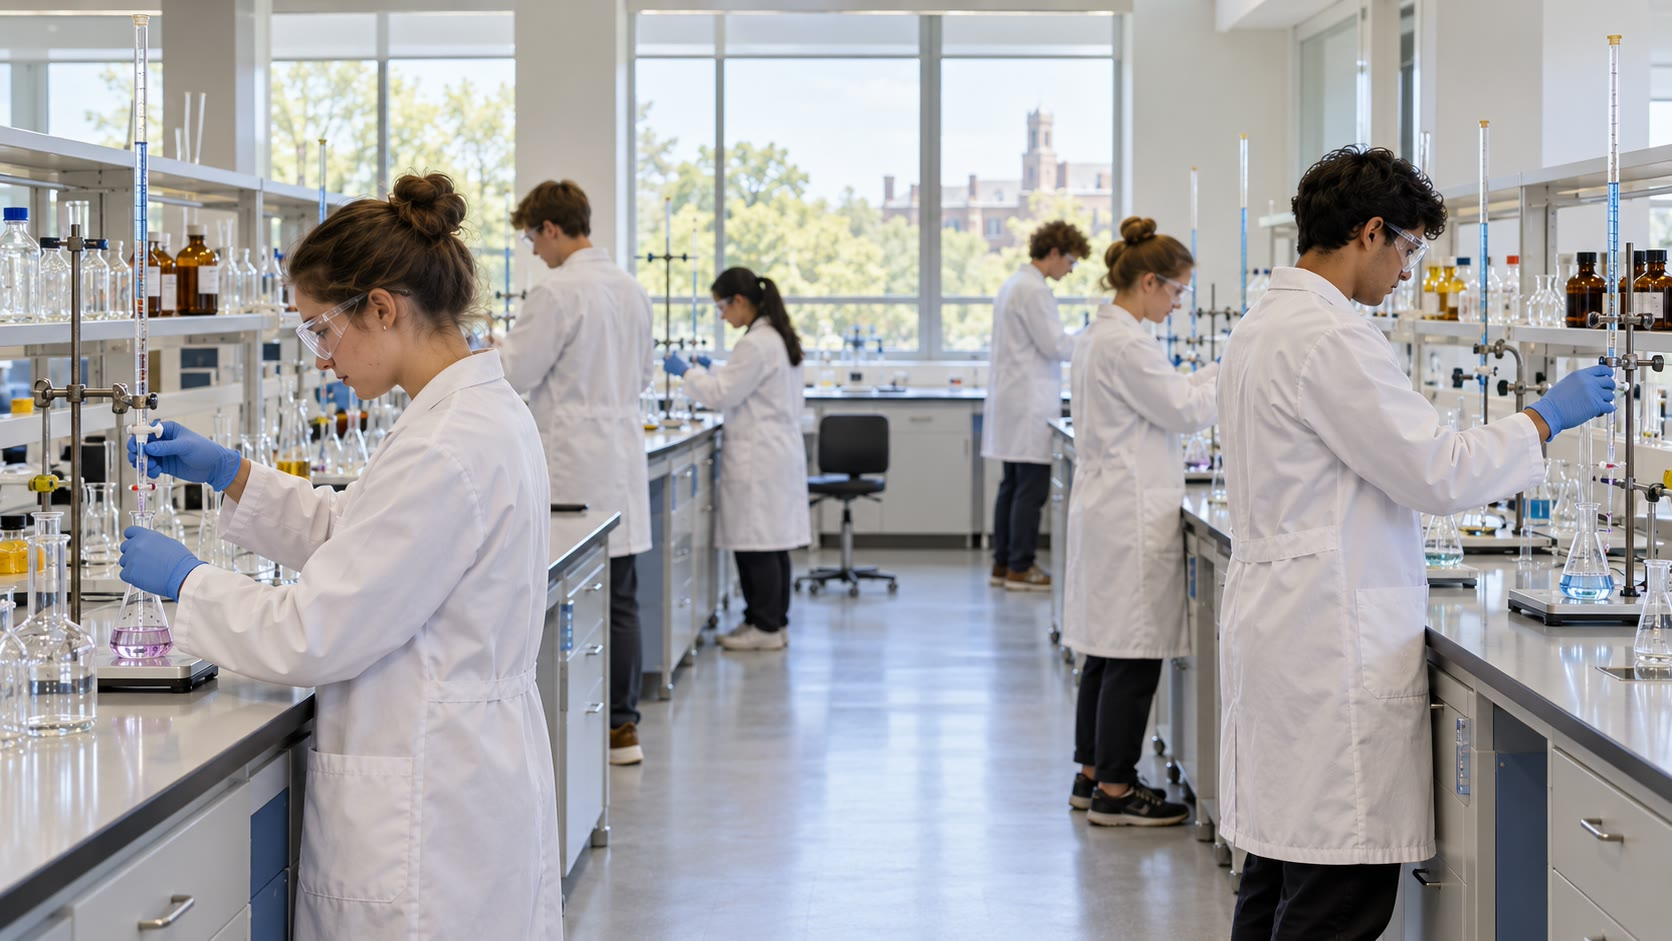
\includegraphics[width=0.66\linewidth]{images/book2/ai/b1-15-teaching-lab.jpg}

{\small Een practicumlokaal: een buret, een erlenmeyer op een
magneetroerder, handschoenen en een veiligheidsbril. Een \omterm{def:b1:titration-methods:titration}{titratie} is de
meest gangbare kwantitatieve meting in de scheikunde.}
\end{omfigure}

\section{Titratie en equivalentie}

\begin{definition}[Titratie, equivalentie]\label{def:b1:titration-methods:titration}
Een \emph{titratie}\index{titratie} bepaalt de hoeveelheid van een
deeltje, het \emph{analiet}\index{analiet}, via een reactie met een
reagens van bekende concentratie, de \emph{titrant}\index{titrant}, dat
geleidelijk wordt toegevoegd. De reactie moet uniek, \omterm{def:b1:extent-q-and-k:quantitative}{kwantitatief} ($K$
groot) en snel zijn. De \emph{equivalentie}\index{equivalentie} is bereikt
wanneer titrant en analiet bij elkaar gebracht zijn in de
stoichiometrische verhoudingen van de reactie; het dan toegevoegde volume
is het equivalentievolume, en het punt van de titratiekromme bij dat
volume is het
\emph{equivalentiepunt}\index{equivalentiepunt}. Het volume waarbij de
experimentator stopt, omdat hij een kleuromslag of een knik in een kromme
ziet, is het \emph{eindpunt}\index{eindpunt}; een goede methode laat het
samenvallen met de equivalentie.
\end{definition}

\begin{proposition}[Equivalentiebetrekking]\label{prop:b1:titration-methods:equivalence}
Voor een titratiereactie $a\,\mathrm{A} + b\,\mathrm{B} \to \cdots$, met
\omterm{def:b1:titration-methods:titration}{analiet} A ($n_A$ mol) en \omterm{def:b1:titration-methods:titration}{titrant} B met concentratie $C_B$, voldoet het
equivalentievolume aan
\[
  \frac{n_A}{a} = \frac{C_B V_{\mathrm{eq}}}{b} .
\]
\end{proposition}

\begin{proof}
Zij $x$ de voortgang na toevoeging van $V$ \omterm{def:b1:titration-methods:titration}{titrant}. Vóór de \omterm{def:b1:titration-methods:titration}{equivalentie}
is B beperkend en, omdat de reactie \omterm{def:b1:extent-q-and-k:quantitative}{kwantitatief} is, $x = C_BV/b$;
daarna is A beperkend en $x = n_A/a$. De \omterm{def:b1:titration-methods:titration}{equivalentie} is het volume
waarbij beide samen op zijn, $n_A - ax = 0$ en $C_BV - bx = 0$: $x$
elimineren geeft de betrekking.
\end{proof}

\section{Directe en indirecte titraties}

\begin{definition}[Soorten titraties]\label{def:b1:titration-methods:kinds}
Bij een \emph{directe titratie}\index{directe titratie} reageert de
\omterm{def:b1:titration-methods:titration}{titrant} met het \omterm{def:b1:titration-methods:titration}{analiet} zelf. Bij een
\emph{terugtitratie}\index{terugtitratie} wordt een bekende overmaat van
een reagens aan het \omterm{def:b1:titration-methods:titration}{analiet} toegevoegd, en wordt de overgebleven
overmaat getitreerd. Wanneer een oplossing meerdere \omterm{def:b1:titration-methods:titration}{analieten} bevat die
na elkaar met de \omterm{def:b1:titration-methods:titration}{titrant} reageren, worden ze bepaald door
\emph{opeenvolgende titraties}\index{opeenvolgende titraties}, de ene
\omterm{def:b1:titration-methods:titration}{equivalentie} na de andere; wanneer ze samen reageren en één enkele
\omterm{def:b1:titration-methods:titration}{equivalentie} geven, door een \emph{gelijktijdige
titratie}\index{gelijktijdige titratie}, die alleen hun som geeft.
\end{definition}

\begin{method}[Terugtitratie]\label{met:b1:titration-methods:back-titration}
Gebruik ze wanneer de directe reactie traag is, wanneer het \omterm{def:b1:titration-methods:titration}{analiet}
instabiel of vluchtig is, of wanneer geen enkele indicator bij de directe
reactie past.
\begin{enumerate}
  \item Voeg een bekende hoeveelheid $n_R$ van het reagens R in overmaat
        toe, en laat het volledig met het \omterm{def:b1:titration-methods:titration}{analiet} A reageren
        ($\alpha\,\mathrm{A} + \rho\,\mathrm{R}$).
  \item Titreer de overmaat R met een \omterm{def:b1:titration-methods:titration}{titrant} T ($\rho'\,\mathrm{R} +
        \tau\,\mathrm{T}$) tot het equivalentievolume $V_T$.
  \item Bereken $n_{R,\text{overmaat}} = \frac{\rho'}{\tau}C_TV_T$, en
        daarna $n_A = \frac{\alpha}{\rho}(n_R - n_{R,\text{overmaat}})$.
\end{enumerate}
\end{method}

Het weekendprobleem titreert vitamine C op deze manier: ascorbinezuur
reduceert een overmaat jood, en het overgebleven jood wordt met
thiosulfaat getitreerd.

\section{pH-metrische titraties en indicatoren}

\begin{omfigure}
\begin{tikzpicture}[font=\small]
  \pic at (0,0) {stirrer};
  \pic at (0,0.18) {beaker={0.55}{omDef!14}};
  \pic at (0.2,2.45) {burette={0.75}{white}};
  \pic at (-0.45,0.45) {probe};
  \pic (m) at (-2.6,3.2) {meter={pH}};
  \draw[thick] (-0.45,3.45) to[out=90, in=0] (m-b);
  \node[anchor=west] at (0.65,6.2) {buret: NaOH, \qty{0.100}{mol/L}};
  \node[anchor=west] at (1.0,1.0) {zuur, $V_0 = \qty{10.0}{mL}$, verdund};
  \draw[<-, omProp, thick] (1.2,-0.25) -- (1.8,-0.25) node[anchor=west, text=black] {magneetroerder};
  \draw[<-, omProp, thick] (-0.62,2.4) -- (-1.5,2.0) node[anchor=east, text=black] {combinatie-elektrode};
\end{tikzpicture}

{\small Een pH-metrische \omterm{def:b1:titration-methods:titration}{titratie}. De gecombineerde glaselektrode meet de
pH na elke toevoeging uit de buret; de roerder mengt de oplossing. De
elektrode wordt vooraf geijkt met twee \omterm{def:b1:predominant-reaction:buffer}{bufferoplossingen}.}
\end{omfigure}

\begin{omfigure}
\begin{tikzpicture}
\begin{axis}[name=s,
  width=0.5\linewidth, height=5.6cm, xmin=0, xmax=20, ymin=0, ymax=14,
  axis x line=bottom, axis y line=left, xlabel={$V$ (mL)}, ylabel={pH},
  xtick={0,5,10,15,20}, ytick={0,2,4,6,8,10,12,14},
  tick label style={font=\small}, label style={font=\small}]
\addplot[omDef, very thick] table[x=V, y=pH] {figdata/out/bachelor-1-titration-curves-strong.dat};
\addplot[omProp, thick] table[x=V, y=pH] {figdata/out/bachelor-1-titration-curves-weak.dat};
\node[font=\scriptsize, omDef, anchor=south west] at (axis cs:6,0.2) {\ce{HCl}};
\node[font=\scriptsize, omProp, anchor=west] at (axis cs:0.4,6.4) {\ce{CH3COOH}};
\draw[dotted] (axis cs:5,0) -- (axis cs:5,4.76) -- (axis cs:0,4.76);
\node[font=\scriptsize, anchor=north] at (axis cs:2.5,4.7) {$\mathrm{p}K_a$};
\end{axis}
\begin{axis}[at={(s.east)}, anchor=west, xshift=1.2cm,
  width=0.5\linewidth, height=5.6cm, xmin=0, xmax=20, ymin=0, ymax=14,
  axis x line=bottom, axis y line=left, xlabel={$V$ (mL)}, ylabel={pH},
  xtick={0,5,10,15,20}, ytick={0,2,4,6,8,10,12,14},
  tick label style={font=\small}, label style={font=\small}]
\addplot[omMeth, very thick] table[x=V, y=pH] {figdata/out/bachelor-1-titration-curves-mixture.dat};
\node[font=\scriptsize, anchor=west, align=left] at (axis cs:10.8,6.0) {\ce{HCl} + \ce{CH3COOH}\\ twee equivalenties};
\end{axis}
\end{tikzpicture}

{\small Links: \qty{10.0}{mL} zoutzuur en ethaanzuur, beide op
\qty{0.100}{mol/L}, getitreerd met natronloog van
\qty{0.100}{mol/L}. Het \omterm{def:b1:predominant-reaction:strong-acid}{zwakke zuur} heeft een buffergebied met pH $=
\mathrm{p}K_a$ bij de halve \omterm{def:b1:titration-methods:titration}{equivalentie} en een \omterm{def:b1:titration-methods:titration}{equivalentiepunt} bij pH
8.73. Rechts: een mengsel, \qty{0.050}{mol/L} van elk zuur: het \omterm{def:b1:predominant-reaction:strong-acid}{sterke
zuur} wordt eerst getitreerd (\omterm{def:b1:titration-methods:titration}{equivalentie} bij \qty{5}{mL}), daarna het
zwakke (\qty{10}{mL}).}
\end{omfigure}

\begin{proposition}[Halve equivalentie van een zwak zuur]\label{prop:b1:titration-methods:half-equivalence}
Wanneer een \omterm{def:b1:predominant-reaction:strong-acid}{zwak zuur} HA met een \omterm{def:b1:predominant-reaction:strong-acid}{sterke base} getitreerd wordt, is bij de
halve \omterm{def:b1:titration-methods:titration}{equivalentie} $\mathrm{pH} = \mathrm{p}K_a$, op voorwaarde dat het
zuur niet te sterk en niet te verdund is ($\mathrm{p}K_a$ ruwweg tussen
4 en 10 bij \qty{0.1}{mol/L}).
\end{proposition}

\begin{proof}
Bij de halve \omterm{def:b1:titration-methods:titration}{equivalentie} heeft de \omterm{def:b1:extent-q-and-k:quantitative}{kwantitatieve reactie}
\ce{HA + OH- -> A- + H2O} de helft van HA omgezet:
$[\mathrm{HA}] = [\mathrm{A^-}]$, en de betrekking van Henderson geeft
$\mathrm{pH} = \mathrm{p}K_a$. De voorwaarde zorgt ervoor dat de reactie
van HA met water en die van $\mathrm{A^-}$ met water die hoeveelheden
niet merkbaar veranderen.
\end{proof}

\begin{proposition}[pH bij de equivalentie van een zwak zuur]\label{prop:b1:titration-methods:ph-at-equivalence}
Bij de \omterm{def:b1:titration-methods:titration}{equivalentie} van een \omterm{def:b1:predominant-reaction:strong-acid}{zwak zuur} ($\mathrm{p}K_a$) met een \omterm{def:b1:predominant-reaction:strong-acid}{sterke
base} is de oplossing de geconjugeerde base met concentratie $C'$ (na
verdunning), en
\[
  \mathrm{pH} = \tfrac12(\mathrm{p}K_e + \mathrm{p}K_a + \log C') .
\]
\end{proposition}

\begin{proof}
De \omterm{def:b1:predominant-reaction:predominant-reaction}{predominante reactie} van de base met water,
\ce{A- + H2O <=> HA + OH-}, heeft $K = K_e/K_a$; als er weinig base
omgezet wordt, is $[\ce{OH-}] = \sqrt{KC'}$
(\cref{prop:b1:predominant-reaction:ph-formulas}), waaruit het resultaat
volgt. Voor ethaanzuur, $C' = \qty{0.050}{mol/L}$:
$\frac12(14.00 + 4.76 - 1.30) = 8.73$.
\end{proof}

\begin{proposition}[Opeenvolgende titraties]\label{prop:b1:titration-methods:successive}
Twee zuren die met dezelfde base getitreerd worden, geven gescheiden
\omterm{def:b1:titration-methods:titration}{equivalenties}, elk tot op beter dan \qty{1}{\percent}, als hun
$\mathrm{p}K_a$-waarden minstens 4 verschillen.
\end{proposition}

\begin{proof}
Bij de eerste \omterm{def:b1:titration-methods:titration}{equivalentie} heeft de reactie van de base $\mathrm{A_1^-}$
met het tweede zuur $\mathrm{HA_2}$, $\mathrm{A_1^-} + \mathrm{HA_2}
\rightleftharpoons \mathrm{HA_1} + \mathrm{A_2^-}$, de constante
$K = 10^{\mathrm{p}K_1 - \mathrm{p}K_2}$. Uitgaande van gelijke
hoeveelheden voldoet de fractie $x$ van het tweede zuur die al
getitreerd is aan $x^2/(1 - x)^2 = K$; voor $x \leqslant 0.01$ is $K
\leqslant 10^{-4}$, dus $\mathrm{p}K_2 - \mathrm{p}K_1 \geqslant 4$.
\end{proof}

Fosforzuur (2.15, 7.21, 12.34) geeft twee duidelijke \omterm{def:b1:titration-methods:titration}{equivalenties}; de
derde gaat verloren in het water van de base. Ethaanzuur gemengd met
zoutzuur (rechts in de figuur) wordt erna getitreerd, omdat het \omterm{def:b1:predominant-reaction:strong-acid}{sterke
zuur} in feite een $\mathrm{p}K_a$ onder 0 heeft.

\begin{method}[Een equivalentie op een kromme bepalen]\label{met:b1:titration-methods:derivative}
\begin{enumerate}
  \item Afgeleide: bereken $\Delta\mathrm{pH}/\Delta V$ tussen
        opeenvolgende punten; de \omterm{def:b1:titration-methods:titration}{equivalentie} ligt bij het maximum ervan.
  \item Raaklijnen: teken aan weerszijden van de sprong twee evenwijdige
        raaklijnen aan de kromme, en de evenwijdige die op gelijke afstand
        van beide ligt; die snijdt de kromme in het \omterm{def:b1:titration-methods:titration}{equivalentiepunt}.
\end{enumerate}
\end{method}

\begin{method}[Raaklijnen, door berekening]\label{met:b1:titration-methods:tangents}
Pas voor een kromme die door een computer geregistreerd is, de punten aan
elke kant van de sprong aan met een gladde functie en neem het
buigpunt; voor een symmetrische sprong (\omterm{def:b1:predominant-reaction:strong-acid}{sterk zuur}, \omterm{def:b1:predominant-reaction:strong-acid}{sterke base}) is het
midden van de sprong bij pH 7 het \omterm{def:b1:titration-methods:titration}{equivalentiepunt}.
\end{method}

\begin{definition}[Kleurindicator, omslagtraject]\label{def:b1:titration-methods:indicator}
Een \emph{kleurindicator}\index{kleurindicator} is een zwak
zuur-basepaar HIn/In$^-$ waarvan de twee vormen verschillende kleuren
hebben. Zijn kleur verandert over het
\emph{omslagtraject}\index{omslagtraject}, het pH-gebied waar geen van
beide vormen duidelijk overheerst, ongeveer
$\mathrm{p}K_{a}(\mathrm{HIn}) \pm 1$.
\end{definition}

\begin{omfigure}
\begin{tabular}{lccl}
\hline
indicator & $\mathrm{p}K_a$ & \omterm{def:b1:titration-methods:indicator}{omslagtraject} & kleuren (zuur / base) \\
\hline
methyloranje & 3.5 & 2.5--4.5 & rood / geel \\
methylrood & 4.8 & 3.8--5.8 & rood / geel \\
fenolrood & 7.9 & 6.9--8.9 & geel / rood \\
thymolblauw (tweede omslag) & 9.2 & 8.2--10.2 & geel / blauw \\
\hline
\end{tabular}

\smallskip
{\small Vier indicatoren, met $\mathrm{p}K_a$-waarden uit een kritische
compilatie van \omterm{def:b1:complexation:formation-constant}{dissociatieconstanten}; de \omterm{def:b1:titration-methods:indicator}{omslagtrajecten} zijn
$\mathrm{p}K_a \pm 1$.}
% ledger: pka:methylorange, pka:methylred, pka:phenolred, pka:thymolblue2
\end{omfigure}


\begin{method}[Een indicator kiezen]\label{met:b1:titration-methods:choose-indicator}
Kies een indicator waarvan het \omterm{def:b1:titration-methods:indicator}{omslagtraject} binnen de verticale sprong
van de kromme ligt, zo dicht mogelijk bij de pH bij de \omterm{def:b1:titration-methods:titration}{equivalentie}. \omterm{def:b1:predominant-reaction:strong-acid}{Sterk
zuur} met \omterm{def:b1:predominant-reaction:strong-acid}{sterke base} (sprong van 3.3 tot 10.7 voor $\pm\qty{0.1}{mL}$
hier): elk van de vier. Ethaanzuur (\omterm{def:b1:titration-methods:titration}{equivalentie} bij 8.73): fenolrood of
thymolblauw; methyloranje zou al lang vóór de \omterm{def:b1:titration-methods:titration}{equivalentie} omslaan.
\end{method}

\section{Potentiometrische titraties}

\begin{definition}[Potentiometrische titratie]\label{def:b1:titration-methods:potentiometric}
Een \emph{potentiometrische titratie}\index{potentiometrische titratie}
volgt de potentiaal van een elektrode in de oplossing tegen een
\omterm{def:b1:nernst:reference-electrode}{referentie-elektrode}, voor een redoxtitratie (platinadraad), een
neerslagtitratie (zilverdraad) of een complexometrische \omterm{def:b1:titration-methods:titration}{titratie}.
\end{definition}

\begin{proposition}[Bijzondere punten van een redoxtitratie]\label{prop:b1:titration-methods:potentiometric-points}
Voor de \omterm{def:b1:titration-methods:titration}{titratie} van $\mathrm{Red_1}$ met $\mathrm{Ox_2}$ volgens
$n_2\,\mathrm{Red_1} + n_1\,\mathrm{Ox_2} \to n_2\,\mathrm{Ox_1} +
n_1\,\mathrm{Red_2}$ (koppels met $n_1$ en $n_2$ elektronen) is $E(V_{\mathrm{eq}}/2) = E^\circ_1$, $E(2V_{\mathrm{eq}}) =
E^\circ_2$, en bij de \omterm{def:b1:titration-methods:titration}{equivalentie}
\[
  E_{\mathrm{eq}} = \frac{n_1E^\circ_1 + n_2E^\circ_2}{n_1 + n_2},
\]
voor koppels waarvan de \omterm{def:b1:nernst:couple}{halfreacties} geen andere deeltjes bevatten (of bij
een pH die de extra termen vast houdt).
\end{proposition}

\begin{proof}
Bij de halve \omterm{def:b1:titration-methods:titration}{equivalentie} is de helft van $\mathrm{Red_1}$ geoxideerd:
$[\mathrm{Ox_1}] = [\mathrm{Red_1}]$, en de \omterm{thm:b1:nernst:nernst}{vergelijking van Nernst} van
koppel 1 geeft $E^\circ_1$. Bij $2V_{\mathrm{eq}}$ is er evenveel
$\mathrm{Ox_2}$ in overmaat als er gereduceerd werd:
$[\mathrm{Ox_2}] = [\mathrm{Red_2}]$, $E = E^\circ_2$. Vermenigvuldig bij
de \omterm{def:b1:titration-methods:titration}{equivalentie} de \omterm{thm:b1:nernst:nernst}{vergelijking van Nernst} van koppel 1 met $n_1$ en die
van koppel 2 met $n_2$ en tel op; de stoichiometrie maakt
$[\mathrm{Ox_1}]/[\mathrm{Red_1}] \cdot [\mathrm{Ox_2}]/[\mathrm{Red_2}] = 1$
(de overgebleven hoeveelheden $\mathrm{Red_1}$ en $\mathrm{Ox_2}$ staan in
dezelfde verhouding als de producten), zodat de logaritmen wegvallen.
\end{proof}

Voor ijzer(II) met permanganaat in zuur van \qty{1}{mol/L} is $n_1 = 1$
en $n_2 =
5$: $E_{\mathrm{eq}} = (0.77 + 5 \times 1.51)/6 = 1.39$~V. De sprong, van
ongeveer 0.8 tot 1.5~V, is zo groot dat het \omterm{def:b1:titration-methods:titration}{eindpunt} scherp is; in de
praktijk is permanganaat zijn eigen indicator, omdat zijn violette kleur
bij de eerste druppel overmaat blijft.

\begin{omfigure}
\begin{tikzpicture}
\begin{axis}[name=p,
  width=0.5\linewidth, height=5.6cm, xmin=0, xmax=20, ymin=0.6, ymax=1.6,
  axis x line=bottom, axis y line=left, xlabel={$V$ (mL)}, ylabel={$E$ (V)},
  xtick={0,5,10,15,20},
  tick label style={font=\small}, label style={font=\small}]
\addplot[omDef, very thick] table[x=V, y=E] {figdata/out/bachelor-1-titration-curves-potentiometric.dat};
\draw[dotted] (axis cs:5,0.6) -- (axis cs:5,0.77) -- (axis cs:0,0.77);
\draw[dotted] (axis cs:10,0.6) -- (axis cs:10,1.39) -- (axis cs:0,1.39);
\node[font=\scriptsize, anchor=south west] at (axis cs:0.2,0.77) {0.77};
\node[font=\scriptsize, anchor=south west] at (axis cs:0.2,1.39) {1.39};
\end{axis}
\begin{axis}[at={(p.east)}, anchor=west, xshift=1.2cm,
  width=0.5\linewidth, height=5.6cm, xmin=0, xmax=20, ymin=0, ymax=4.6,
  axis x line=bottom, axis y line=left, xlabel={$V$ (mL)},
  ylabel={$\kappa$ (mS/cm)}, xtick={0,5,10,15,20},
  tick label style={font=\small}, label style={font=\small}]
\addplot[omProp, very thick] table[x=V, y=kappa] {figdata/out/bachelor-1-titration-curves-conductimetric.dat};
\draw[dotted] (axis cs:10,0) -- (axis cs:10,1.15);
\end{axis}
\end{tikzpicture}

{\small Links: \omterm{def:b1:titration-methods:potentiometric}{potentiometrische titratie} van \qty{10.0}{mL} ijzer(II)
van \qty{0.100}{mol/L} met permanganaat van \qty{0.0200}{mol/L} in zuur
van \qty{1}{mol/L} (platina-elektrode, potentiaal tegen de
waterstofelektrode). Rechts: conductometrische \omterm{def:b1:titration-methods:titration}{titratie} van
\qty{100}{mL} zoutzuur van \qty{0.0100}{mol/L} met natronloog van
\qty{0.100}{mol/L}; de \omterm{def:b1:titration-methods:titration}{equivalentie} ligt op het snijpunt van twee
rechten.}
% ledger: lam:H+, lam:OH-, lamsalt:HCl, lamsalt:NaCl (conductivities in figdata/bachelor-1/titration-curves.py)
\end{omfigure}


\section{Conductometrische, complexometrische en neerslagtitraties}

\begin{definition}[Molaire ionengeleidbaarheid]\label{def:b1:titration-methods:conductivity}
Het geleidingsvermogen $\kappa$ van een oplossing (in \unit{S/m}) meet
hoe goed ze stroom geleidt door de beweging van haar ionen. De
\emph{molaire ionengeleidbaarheid}\index{molaire ionengeleidbaarheid}
$\lambda_i$ van een ion is zijn bijdrage per mol per volume-eenheid; de
waarde ervan bij oneindige verdunning, $\lambda_i^\circ$, is een
constante van het ion en het oplosmiddel bij een gegeven temperatuur.
\end{definition}

\begin{proposition}[Wet van Kohlrausch]\label{prop:b1:titration-methods:kohlrausch}
In verdunde oplossing is het geleidingsvermogen de som van de bijdragen
van de ionen,
\[
  \kappa = \sum_i \lambda_i^\circ c_i ,
\]
de \emph{wet van Kohlrausch}\index{wet van Kohlrausch}; de molaire
geleidbaarheid van een zout is de som van die van zijn ionen.
\end{proposition}

\admitted{De \omterm{prop:b1:titration-methods:kohlrausch}{wet van Kohlrausch} drukt uit dat verdunde ionen zich
onafhankelijk van elkaar bewegen; haar grenzen bij hogere concentratie
worden bestudeerd in het deel van jaar~2. We gebruiken haar hier als een
experimentele wet.}

\begin{proposition}[Hellingen van een conductometrische titratie]\label{prop:b1:titration-methods:conductimetric-slopes}
Wanneer een \omterm{def:b1:predominant-reaction:strong-acid}{sterk zuur} H$^+$X$^-$ getitreerd wordt met een \omterm{def:b1:predominant-reaction:strong-acid}{sterke base}
Na$^+$OH$^-$ in een groot volume (verdunning verwaarloosd), varieert het
geleidingsvermogen lineair met het toegevoegde volume, met een helling
die evenredig is met
$\lambda^\circ(\ce{Na+}) - \lambda^\circ(\ce{H+}) < 0$ vóór de
\omterm{def:b1:titration-methods:titration}{equivalentie} en met $\lambda^\circ(\ce{Na+}) + \lambda^\circ(\ce{OH-}) > 0$
erna.
\end{proposition}

\begin{proof}
Vóór de \omterm{def:b1:titration-methods:titration}{equivalentie} verwijdert elke toegevoegde mol hydroxide één mol
\ce{H+} (\ce{H+ + OH- -> H2O}) en brengt ze één mol \ce{Na+} in; na de
\omterm{def:b1:titration-methods:titration}{equivalentie} voegt ze één \ce{Na+} en één \ce{OH-} toe. \ce{X-} blijft
ongewijzigd. Volgens de \omterm{prop:b1:titration-methods:kohlrausch}{wet van Kohlrausch} verandert het
geleidingsvermogen met die combinaties van $\lambda^\circ$, maal de
toegevoegde hoeveelheid gedeeld door het (vaste) volume.
\end{proof}

Uit de grensgeleidbaarheden, $\lambda^\circ(\ce{H+}) =
\qty{349.8}{S.cm^2/mol}$ en $\lambda^\circ(\ce{OH-}) = 198.3$, en die
van de zouten \ce{HCl} (426) en \ce{NaCl} (126.5), geeft de \omterm{prop:b1:titration-methods:kohlrausch}{wet van
Kohlrausch} $\lambda^\circ(\ce{Cl-}) = 426 - 349.8 = 76.2$ en
$\lambda^\circ(\ce{Na+}) =
126.5 - 76.2 = 50.3$~\unit{S.cm^2/mol}. De waterstof- en hydroxide-ionen
geleiden veel beter dan de andere: de kromme is een scherpe V.

Complexometrische \omterm{def:b1:titration-methods:titration}{titraties} gebruiken edta: bij pH 10 (ammoniakbuffer)
reageren calcium en magnesium er \omterm{def:b1:extent-q-and-k:quantitative}{kwantitatief} mee (conditionele
constanten van \cref{ch:b1:complexation}), en een indicator die zelf een
zwakke complexvormer van het metaal is, verandert van kleur wanneer edta
er de laatste metaalionen van afneemt --- de \omterm{def:b1:titration-methods:titration}{titratie} van de
waterhardheid. Neerslagtitraties gebruiken zilverionen: chloride wordt
getitreerd met zilvernitraat met chromaat als indicator
(\cref{exo:b1:precipitation:8}), of gevolgd met een zilverelektrode
(\cref{ch:b1:nernst}). De nauwkeurigheid van al die resultaten, bepaald
door het glaswerk en het \omterm{def:b1:titration-methods:titration}{eindpunt}, wordt behandeld in
\cref{ch:b1:lab-techniques-1}.

\section{Oefeningen}

\begin{exercise}[$\star$]\label{exo:b1:titration-methods:1}
\qty{20.0}{mL} van een natronloogoplossing vereist \qty{12.4}{mL}
zoutzuur van \qty{0.100}{mol/L}. Schrijf de reactie op en haar
constante, en bereken de concentratie van de base.
\end{exercise}

\begin{exercise}[$\star$]\label{exo:b1:titration-methods:2}
Welke indicator uit de tabel past bij de \omterm{def:b1:titration-methods:titration}{titratie} van ammoniak
(\qty{0.10}{mol/L}, $\mathrm{p}K_a = 9.25$) met zoutzuur van
\qty{0.10}{mol/L}? Bereken eerst de pH bij de \omterm{def:b1:titration-methods:titration}{equivalentie}.
\end{exercise}

\begin{exercise}[$\star$]\label{exo:b1:titration-methods:3}
\qty{10.0}{mL} ijzer(II) wordt getitreerd met permanganaat van
\qty{0.0200}{mol/L}; de violette kleur blijft vanaf \qty{12.6}{mL}.
Schrijf de reactie op en bereken de concentratie van ijzer(II).
\end{exercise}

\begin{exercise}[$\star$]\label{exo:b1:titration-methods:4}
Een watermonster van \qty{50.0}{mL} wordt bij pH 10 getitreerd met edta
van \qty{0.0100}{mol/L}; de \omterm{def:b1:titration-methods:titration}{equivalentie} ligt bij \qty{14.2}{mL}. Edta
reageert één op één met calcium en magnesium. Bereken de totale
concentratie van deze twee ionen. Is dit een gelijktijdige of een
opeenvolgende \omterm{def:b1:titration-methods:titration}{titratie}?
\end{exercise}

\begin{exercise}[$\star\star$]\label{exo:b1:titration-methods:5}
Bereken voor de \omterm{def:b1:titration-methods:titration}{titratie} van \qty{10.0}{mL} ethaanzuur van
\qty{0.100}{mol/L} met natronloog van \qty{0.100}{mol/L} de pH bij 0,
5.0, 10.0 en \qty{15.0}{mL} met de methoden van
\cref{ch:b1:predominant-reaction}, en vergelijk met de kromme van dit
hoofdstuk.
\end{exercise}

\begin{exercise}[$\star\star$]\label{exo:b1:titration-methods:6}
Toon aan dat een pH-metrische \omterm{def:b1:titration-methods:titration}{titratie} van fosforzuur met natronloog
twee sprongen geeft, en bereken de pH bij elke \omterm{def:b1:titration-methods:titration}{equivalentie} voor een zuur
van \qty{0.100}{mol/L} (\qty{10.0}{mL}, base \qty{0.100}{mol/L}). Waarom
is er geen derde sprong?
\end{exercise}

\begin{exercise}[$\star\star$]\label{exo:b1:titration-methods:7}
Een mengsel van zoutzuur en ethaanzuur (\qty{10.0}{mL}) wordt getitreerd
met natronloog van \qty{0.100}{mol/L}: twee \omterm{def:b1:titration-methods:titration}{equivalenties}, bij
\qty{6.2}{mL} en \qty{14.6}{mL}. Bereken de twee concentraties. Wat is de
pH halverwege de twee \omterm{def:b1:titration-methods:titration}{equivalenties}?
\end{exercise}

\begin{exercise}[$\star\star$]\label{exo:b1:titration-methods:8}
Bereken de potentiaal van de platina-elektrode bij de \omterm{def:b1:titration-methods:titration}{titratie} van
ijzer(II) met permanganaat (gegevens uit het hoofdstuk) bij 2.0, 9.0,
11.0 en \qty{20.0}{mL}.
\end{exercise}

\begin{exercise}[$\star\star$]\label{exo:b1:titration-methods:9}
Bereken met de \omterm{prop:b1:titration-methods:kohlrausch}{wet van Kohlrausch} en de waarden uit het hoofdstuk het
geleidingsvermogen van het getitreerde zoutzuur bij 0, 10.0 en
\qty{20.0}{mL} base (\qty{100}{mL} zuur van \qty{0.0100}{mol/L}, base
van \qty{0.100}{mol/L}, met inbegrip van de verdunning), en de twee
hellingen.
\end{exercise}

\begin{exercise}[$\star\star\star$]\label{exo:b1:titration-methods:10}
Bewijs dat de pH-metrische kromme van een \omterm{def:b1:predominant-reaction:strong-acid}{sterk zuur} dat met een \omterm{def:b1:predominant-reaction:strong-acid}{sterke
base} getitreerd wordt, symmetrisch is ten opzichte van het
\omterm{def:b1:titration-methods:titration}{equivalentiepunt} wanneer de verdunning verwaarloosd wordt, en bereken de
grootte van de sprong tussen $V_{\mathrm{eq}} \pm 0.1$~mL voor de
\omterm{def:b1:titration-methods:titration}{titratie} van het hoofdstuk. Hoe verandert ze als alle concentraties door
100 gedeeld worden?
\end{exercise}

\begin{exercise}[$\star\star\star$]\label{exo:b1:titration-methods:11}
Leid de vergelijking af van de potentiometrische kromme van ijzer(II)
met permanganaat vóór en na de \omterm{def:b1:titration-methods:titration}{equivalentie}, en controleer de drie
bijzondere punten van
\cref{prop:b1:titration-methods:potentiometric-points}. Hoe zou de
potentiaal bij de \omterm{def:b1:titration-methods:titration}{equivalentie} veranderen bij pH 1?
\end{exercise}

\begin{exercise}[$\star\star\star$]\label{exo:b1:titration-methods:12}
Ammoniumchloride (\qty{0.100}{mol/L}, $\mathrm{p}K_a = 9.25$) kan niet
nauwkeurig met natronloog getitreerd worden met een indicator. Verklaar
aan de hand van de kromme, en stel daarna een \omterm{def:b1:titration-methods:kinds}{terugtitratie} voor: een
overmaat natronloog, de ammoniak wegkoken, de overgebleven hydroxide
titreren met zoutzuur. Schrijf de berekening op.
\end{exercise}

\section{Probleem: hoeveel vitamine C zit er in de tablet?}

\begin{problem}[{Weekendprobleem --- de reactie van jood met
ascorbinezuur, een terugtitratie met thiosulfaat, de berekening van het
resultaat en zijn onzekerheid, met als eindpunt de massa ascorbinezuur
per tablet}]
\label{pb:b1:titration-methods:1}
Een tablet wordt fijngemaakt en in water opgelost in een maatkolf van
\qty{100.0}{mL}. Met een pipet wordt een deel van \qty{10.00}{mL}
genomen, en er wordt \qty{20.00}{mL} joodoplossing van
\qty{0.0250}{mol/L} toegevoegd (overmaat). Het overgebleven jood wordt
getitreerd met natriumthiosulfaat van \qty{0.0500}{mol/L} met zetmeel als
indicator: de blauwe kleur verdwijnt bij \qty{8.90}{mL}. Ascorbinezuur is
\ce{C6H8O6} ($M = \qty{176.0}{g/mol}$); jood oxideert het tot
\ce{C6H6O6}. $E^\circ(\ce{I2}/\ce{I-}) = 0.53$~V,
$E^\circ(\ce{S4O6^2-}/\ce{S2O3^2-}) = 0.02$~V.

\medskip
\noindent\textbf{Deel I --- De reacties.}
\begin{enumerate}
  \item Schrijf de \omterm{def:b1:nernst:couple}{halfreactie} op van het koppel \ce{C6H6O6}/\ce{C6H8O6}.
  \item Schrijf de reactie van jood met ascorbinezuur op.
  \item Geef het \omterm{def:b1:nernst:oxidation-number}{oxidatiegetal} van jood in \ce{I2} en \ce{I-}.
  \item Schrijf de reactie van jood met thiosulfaat op en bereken haar
        constante.
  \item Zetmeel geeft met jood een diepblauwe kleur. Waarom verdwijnt de
        kleur precies bij de \omterm{def:b1:titration-methods:titration}{equivalentie} van de \omterm{def:b1:titration-methods:titration}{titratie} met
        thiosulfaat?
  \item Ascorbinezuur wordt langzaam geoxideerd door de zuurstof van de
        lucht. Waarom pleit dat ervoor het jood meteen en in overmaat toe
        te voegen?
\end{enumerate}

\medskip
\noindent\textbf{Deel II --- Waarom een \omterm{def:b1:titration-methods:kinds}{terugtitratie}?}
\begin{enumerate}[resume]
  \item Wat zou een \omterm{def:b1:titration-methods:kinds}{directe titratie} van ascorbinezuur met jood vereisen?
  \item Beschrijf de \omterm{def:b1:titration-methods:kinds}{terugtitratie} als de drie stappen van
        \cref{met:b1:titration-methods:back-titration}.
  \item Waarom moet het jood in overmaat zijn? Controleer het met het
        resultaat.
  \item Waarom wordt de thiosulfaatoplossing kort voor gebruik
        gestandaardiseerd?
  \item Het genomen deel is \qty{10.00}{mL} van \qty{100.0}{mL}: wat is de
        verdunningsfactor?
  \item Met welk glaswerk worden de \qty{20.00}{mL} joodoplossing
        afgemeten?
\end{enumerate}

\medskip
\noindent\textbf{Deel III --- De berekening.}
\begin{enumerate}[resume]
  \item Bereken de ingebrachte hoeveelheid jood.
  \item Bereken de verbruikte hoeveelheid thiosulfaat.
  \item Leid de hoeveelheid jood in overmaat af.
  \item Leid de hoeveelheid jood af die met ascorbinezuur gereageerd
        heeft.
  \item Bereken de hoeveelheid ascorbinezuur in het genomen deel.
  \item Bereken de hoeveelheid, en daarna de massa, ascorbinezuur in de
        tablet.
  \item Vergelijk met het etiket (\qty{500}{mg}).
\end{enumerate}

\medskip
\noindent\textbf{Deel IV --- Hoe zeker?}
De toleranties zijn: maatkolf \qty{100.0 \pm 0.1}{mL}, pipetten
\qty{10.00 \pm 0.02}{mL} en \qty{20.00 \pm 0.03}{mL}, aflezing van de
buret $\pm\qty{0.05}{mL}$; de twee concentraties zijn bekend tot op
\qty{0.2}{\percent}.
\begin{enumerate}[resume]
  \item Druk $n(\text{ascorbinezuur})$ in de tablet uit als functie van
        de gemeten grootheden.
  \item Welke relatieve onzekerheden spelen mee in de ingebrachte
        hoeveelheid jood en in de hoeveelheid in overmaat?
  \item Waarom vergroot een verschil van twee hoeveelheden de relatieve
        onzekerheid?
  \item Schat, door de bijdragen te combineren zoals in
        \cref{ch:b1:lab-techniques-1} (kwadratische som), de relatieve
        onzekerheid van het resultaat.
  \item Geef de massa ascorbinezuur per tablet met haar onzekerheid, op
        twee beduidende cijfers.
\end{enumerate}
\end{problem}
